In order to assess our extension in a variety of different situations we ran several simulations. We looked to replicate different types of node behaviour and then assess different PAC strategies on each. Importantly, we introduced churn into the simulated networks. Our analysis so far has not accounted for churn, where nodes leave the network and so decrease awareness. These simulations, therefore, demonstrate our extension's effectiveness in a more true-to-life environment.

\subsection{The Design}

    The simulation software was written in Java and is publicly hosted on GitHub\footnote{\url{https://github.com/WilliamMayor/SimPact}}. The software simulates nodes in a peer to peer network, each making independent decisions about their search, download and upload behaviours. A round of the simulation consists of every node making a single action, these actions could be to start searching for or downloading a torrent, to leave the network, or simply to remain in the network. Each round is considered to take unit time. After each round, each node is quizzed regarding its state and the responses are stored. Rounds continue until there is no possibility of a successful download, this could be because all participants in the torrent have left, or perhaps because there is no awareness of the torrent in the network. A single trial of the simulation consists of a complete set of rounds. At the end of a trial the data gathered from each of the nodes in each of the rounds is collected and an average value for each statistic at each round is stored. Trials continue until either the minimum number has been run or we have obtained a 5\% confidence interval for each of the statistics calculated, whichever is larger.

    For our simulations we implemented two distinct patterns of node behaviour. One is based on the fluid model of peer to peer nodes developed in \cite{Qiu2004,Guo2007}. A node's behaviour is decided according to which of four states the node is in; passive, downloading, seeding and dead. A passive node does not interact with a torrent directly but does respond to PAC search requests by building and maintaining a local index. All nodes are initialised as passive nodes, passive nodes can either remain passive for their lifetime or can instead be chosen to initiate a search. If a passive node has been chosen to become a downloading node then when it is initialised it decides a waiting time by sampling from an exponential distribution that models node arrival time. The parameters to the distribution can be tailored to suit the simulation. At each round the passive node decreases the wait time, when the time reaches zero the node performs a PAC search and becomes a downloading node. Downloading nodes remain available for PAC requests but at each round there are now two state checks to perform. The first is the download abort check, this is a waiting time, much like the passive node's arrival time, that is sampled from a different exponential distribution. If the abort time reaches zero then the node moves into the dead state. The second check is to see if the download has completed, this check involves increasing the download complete percentage. The percentage increase at each round depends on the node's available download bandwidth and the collective upload bandwidth available from other, participating, nodes. If the download complete percentage reaches 100 before the abort time reaches zero then the node becomes a seeding node. Seeding nodes remain available for PAC search requests and contribute to the total available upload bandwidth in the network. At each round they decrease their seeding wait time, sampled from a third exponential distribution. If the seeding time reaches zero then the node becomes a dead node. A dead node is one that has left the network and is no longer available for requests. When a node leaves the network it is replaced by a fresh node in order to keep the network size constant. The fresh node shares no data with the departing node and they have differing network addresses. Passive nodes enter and leave the network according to the same behaviours as described above. The difference is that their status is not recorded. This is done in order to simulate network churn.

    The second pattern of node behaviour is one described in \cite{Zhang2011}. The authors observe that a proportion of torrents display a constant popularity. We model this behaviour in two ways, the first is to keep a static number of nodes in the seeding state, the second is to churn the torrent's participants by adding a new node to the torrent every time an older one leaves. For both constant popularity models the passive nodes exhibit the same churn behaviour as before.

    We ran 72 simulations, each for a minimum of 500 trials. We tuned the simulations to produce 18 different types of node behaviour and for each type we tested four different strategies for PAC search. In each simulation we fixed the network size to 5 million nodes and we simulated and observed a single torrent. A limit was set on the total lifetime torrent popularity, the maximum number of nodes that ever participate in the torrent. This was done to limit the runtime of the simulations and to help shape the popularity over time. For fluid model simulations we considered four different popularity shapes; large, medium, small and extra small. These were defined by the peak popularity over the torrent's lifetime. Large torrents peaked at 10,000 concurrently participating nodes, medium at 5,000, small at 1,000 and extra at only 100, see Figure~\ref{fig:types} for an example. Additionally, fluid model simulations could exhibit standard, flash crowd or long tail node behaviours. In flash crowd simulations nodes seeded the torrent for less time than standard simulations. In long tail simulations nodes seeded for much longer, see Figure~\ref{fig:scales} for an example. Constant model simulations were either; large, with 1,000 participating nodes; medium, with 100; or small with 10. For each type of simulation we then considered the four different PAC strategies seen previously: $z=100, r(1)=1000$, $z=500, r(1)=1000$, $z=500, r(1)=5000$, and $z=1000, r(1)=5000$.

    \begin{figure}[t]
        \centering
        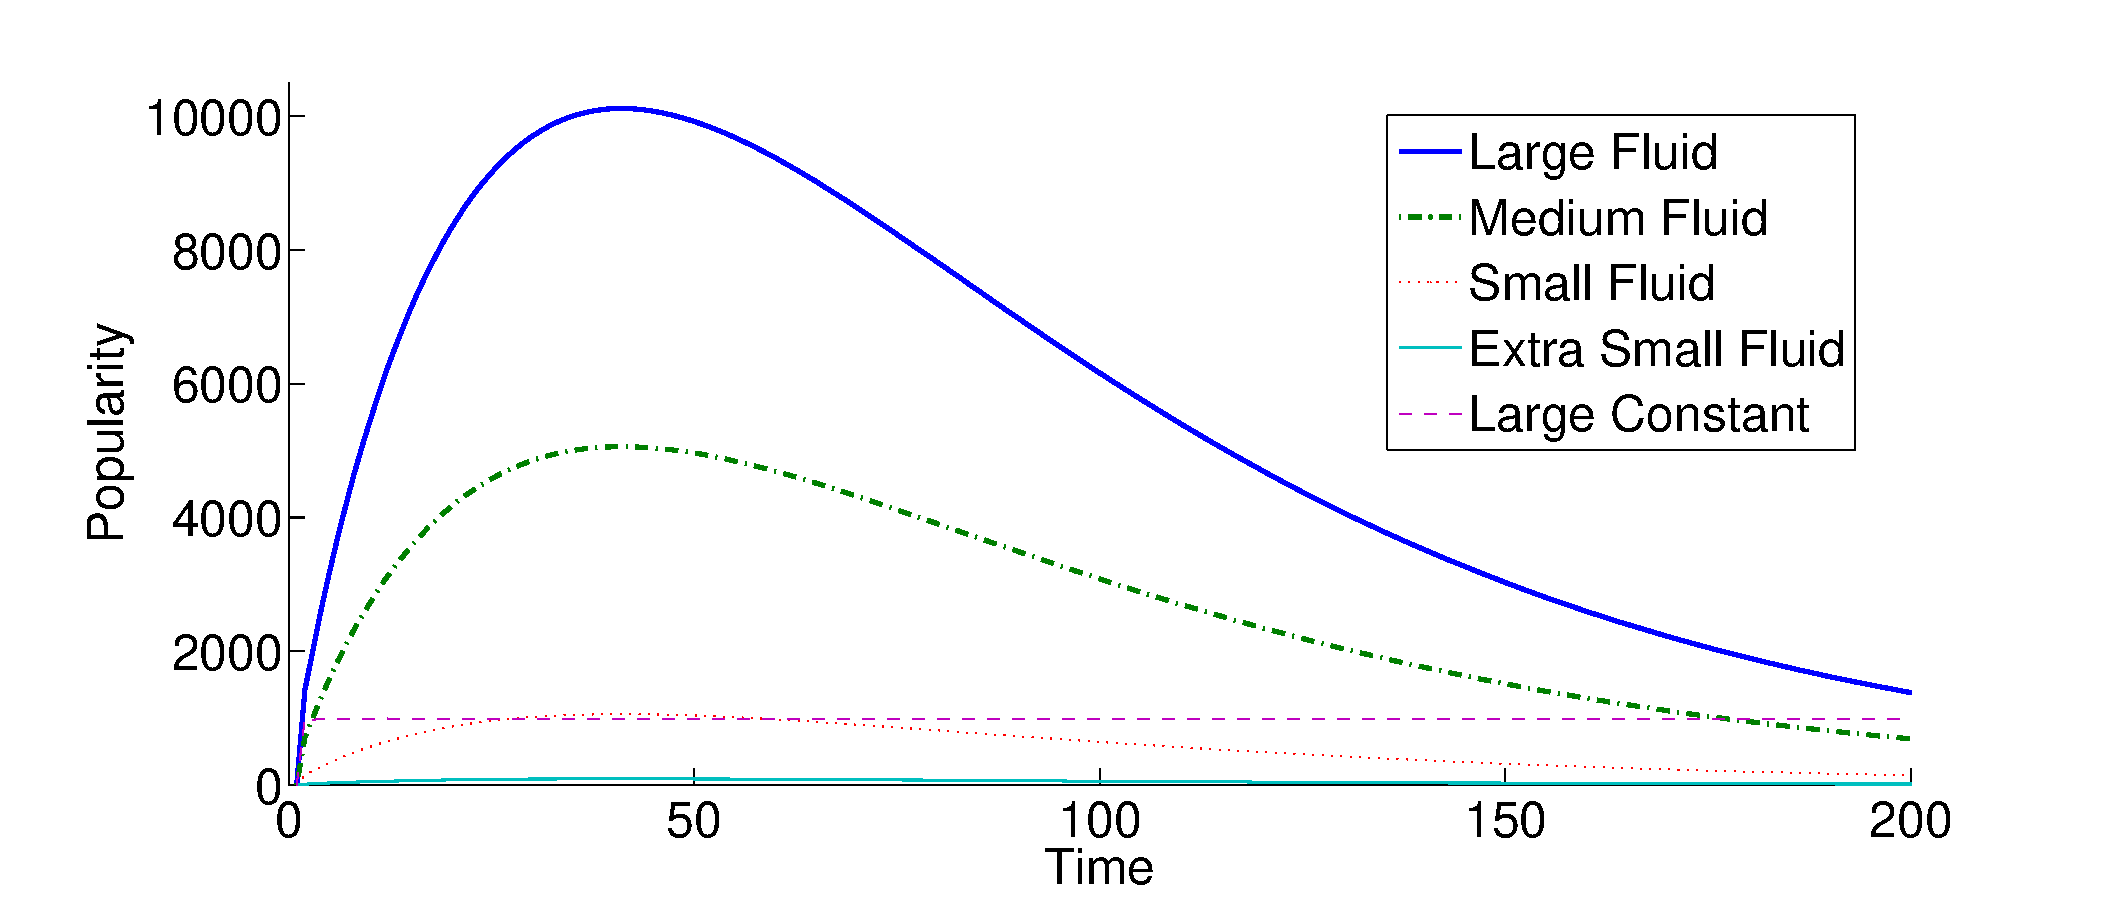
\includegraphics[width=0.5\textwidth]{Images/SimulatedPopularitiesTypes.eps}
        \caption[Popularity over time in five simulation types]{The popularity over time of torrent in five different simulation types.}
        \label{fig:types}
    \end{figure}

    \begin{figure}[t]
        \centering
        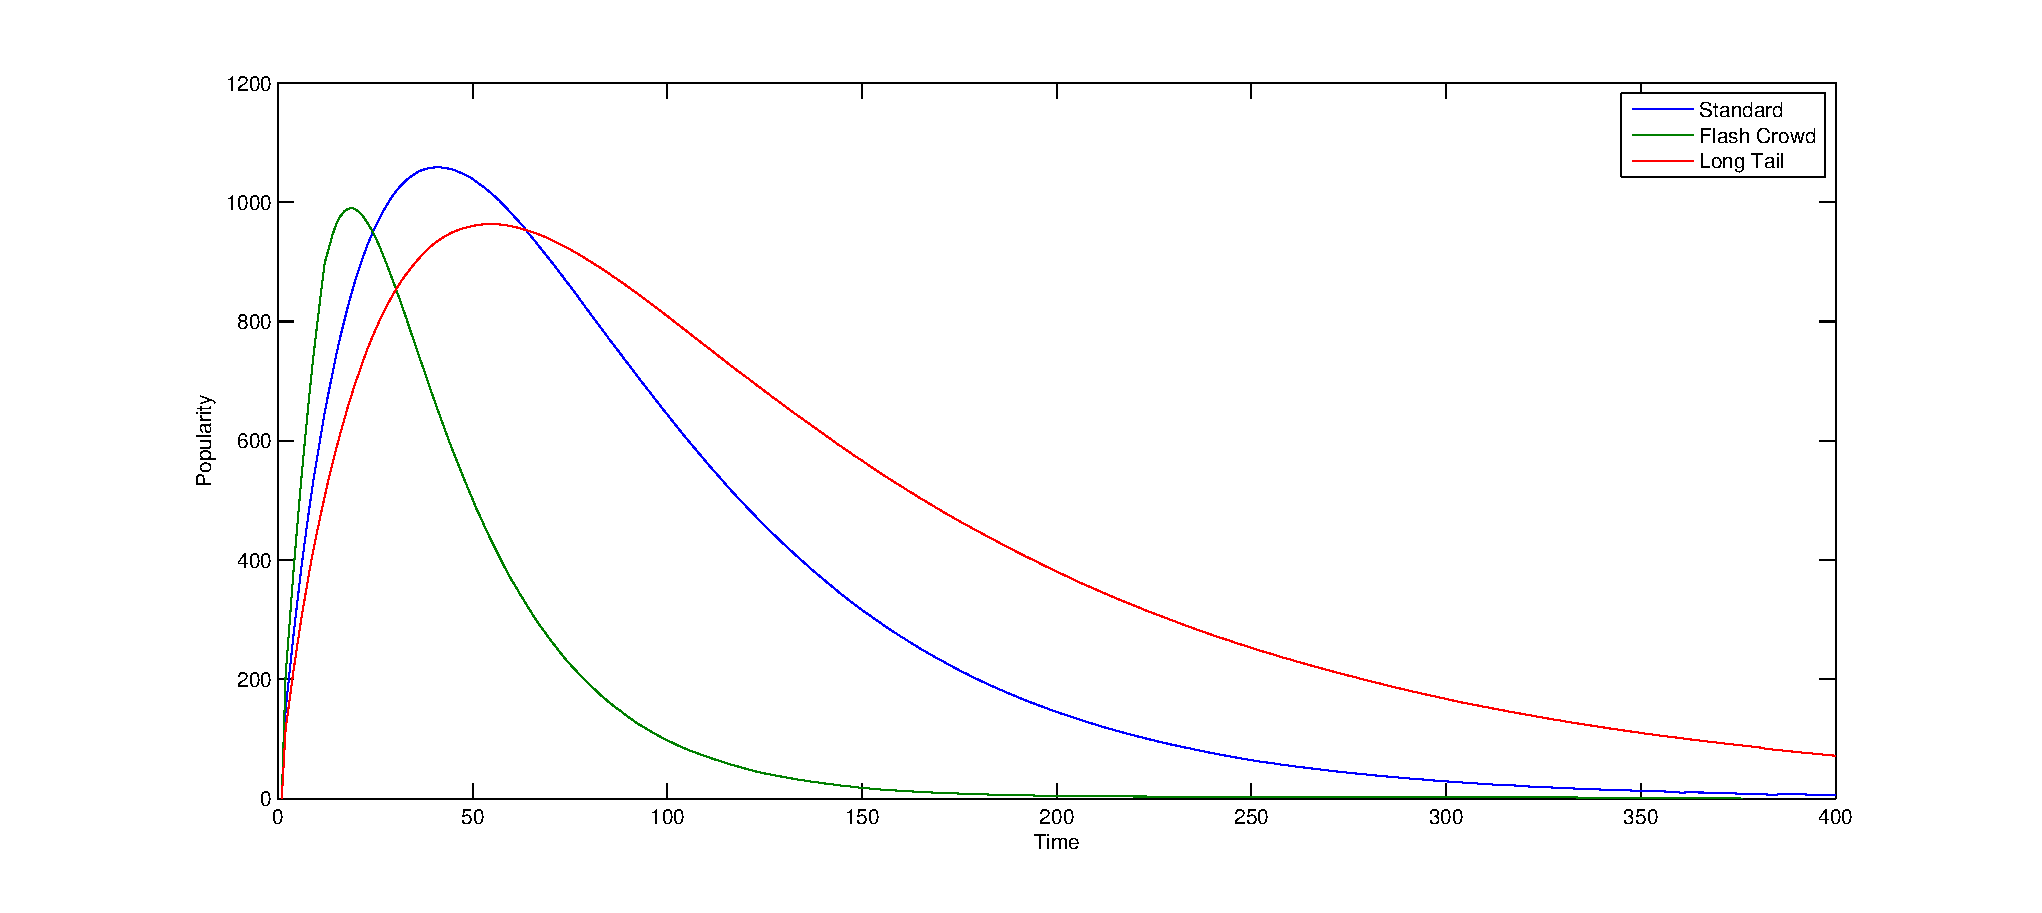
\includegraphics[width=0.5\textwidth]{Images/SimulatedPopularitiesScales.eps}
        \caption[Popularity over time for different scales]{The popularity over time of torrents with different peak popularity.}
        \label{fig:scales}
    \end{figure}

\subsection{The Results}
    
    Figure~\ref{fig:probabilities} shows the probability of a successful query over time for a small sized fluid model simulation. The results displayed use a PAC strategy of $z=100$ and $r(1)=1000$. Simulations of torrents with higher popularity display similar curves with a higher peak, lower popularity torrents display a smaller peak. Likewise when the PAC strategy uses higher values of $z$ or $r(1)$. The probability of a successful query increases and decreases with popularity. This means that, taking into account \emph{when} a query is likely to be performed, we see average probabilities of success over 80\% for every simulation type. There is always a strategy of PAC search that provides a high probability of success, no matter how low the popularity of the torrent. Torrents that display a long-tailed popularity behave as expected; the probability reaches a similar peak at a similar time but remains higher for longer. Long-tailed torrents have a higher average probability of successful search. Torrents that demonstrate a flash-crowd popularity show interesting behaviour towards the end of the simulation; the probability of successful search starts to  fluctuate. This is due to nodes searching for the torrent in a round where the awareness of the torrent is not high enough to easily support it. Those nodes are having to perform several queries repeatedly in order to discover the torrent and so are having a huge impact on the awareness of the torrent. When those late nodes leave the network, the awareness of the torrent subsequently drops by a large amount. Despite this, the average probability of successful search only drops below 70\% in one case out of 16; where torrent popularity peaks at 325, $z=100$ and $r(1)=1000$, in this case the average is 27\%.

    For torrents that exhibit constant popularity we observe some interesting properties that can be exploited. For torrents with static participation the awareness of the torrent decreases only with the churn of the network. As aware nodes leave the network the probability of finding the torrent falls. To counter this decrease, the participating nodes can easily perform additional dummy queries, as when bootstrapping the torrent. If network churn is accurately modelled then an exact figure for the amount of dummy queries required can be calculated and the probability of a successful query can be easily maintained. For torrents with constant, but churning, participation we observe that awareness of the torrent remains as static as the popularity. This is because the steady stream of queries generating awareness offsets the network churn that decreases it. Figure~\ref{fig:constant_probabilities} shows the probability of successful search over time for constant popularity torrents with churning and static participation of large, medium and small sizes.

    \begin{figure}[t]
        \centering
        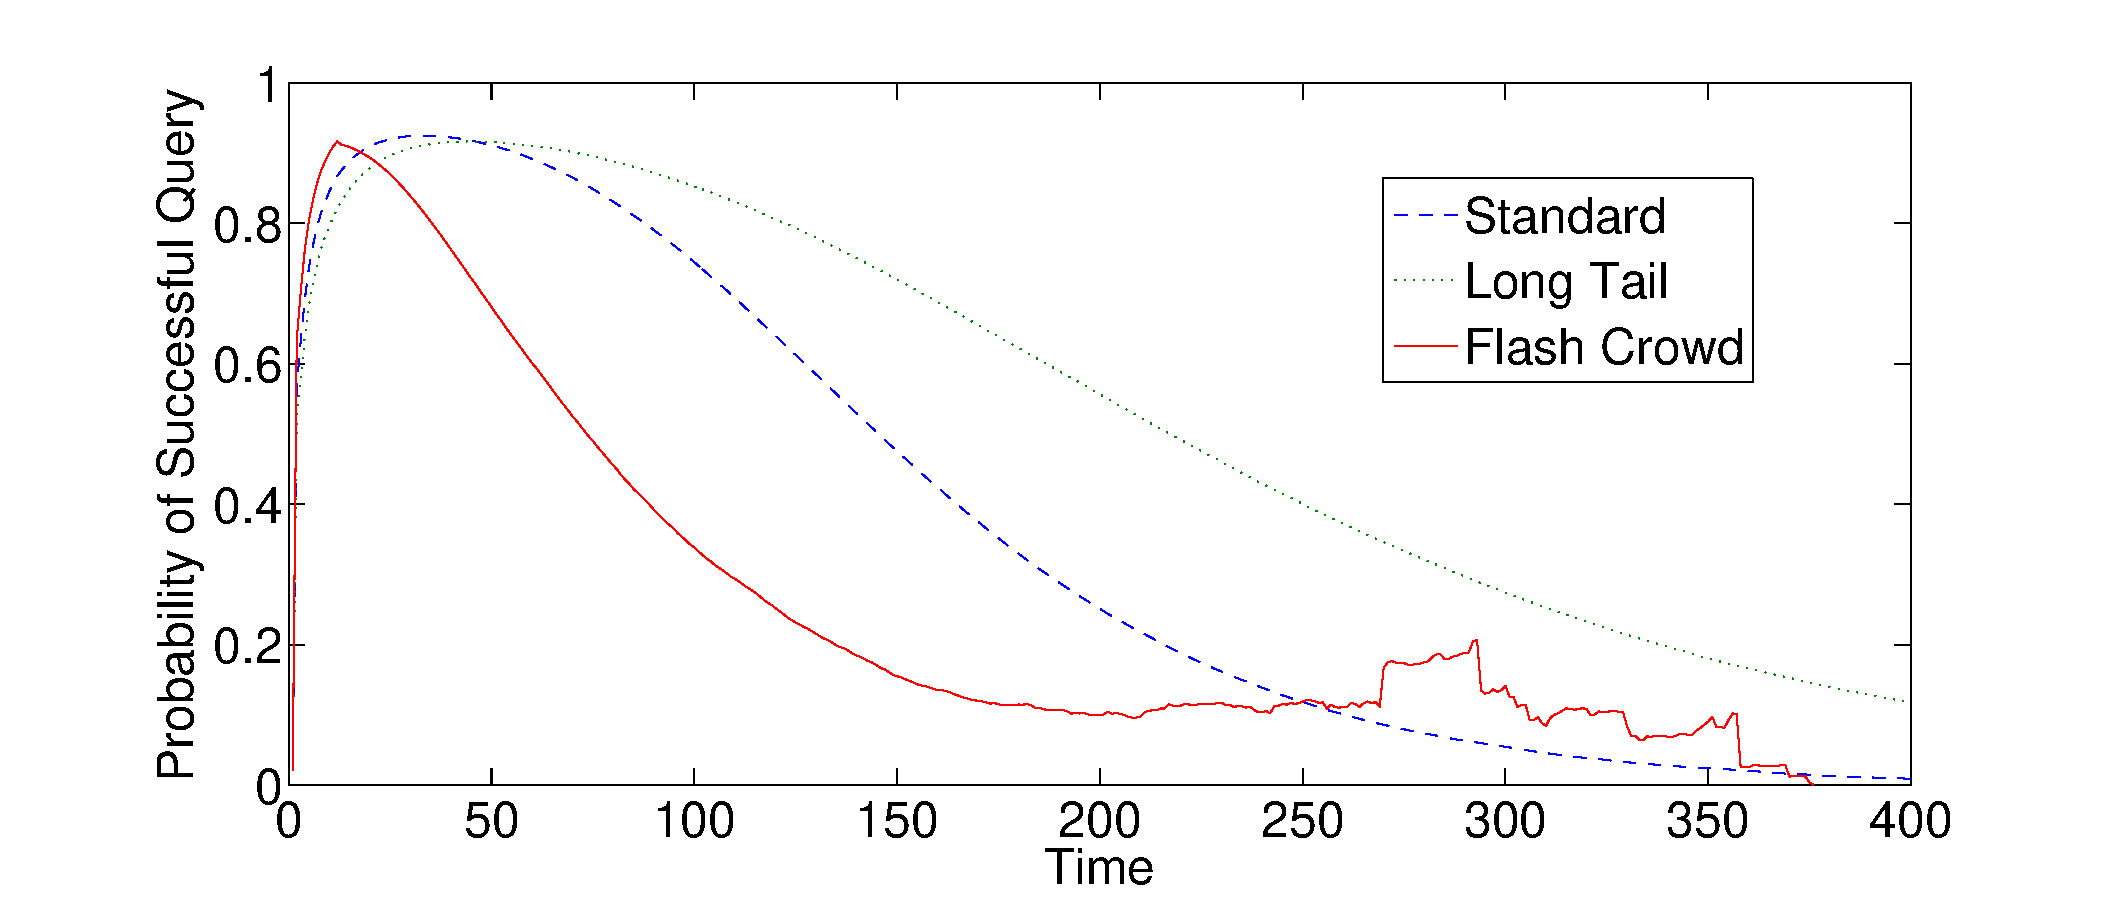
\includegraphics[width=0.5\textwidth]{Images/SimulatedProbabilities.eps}
        \caption{The probability of successful search over time for fluid model popularities. Standard, long-tail and flash crowd torrents are show, each using a PAC strategy of $z=100$ and $r(1)=1000$.}
        \label{fig:probabilities}
    \end{figure}

    \begin{figure}[t]
        \centering
        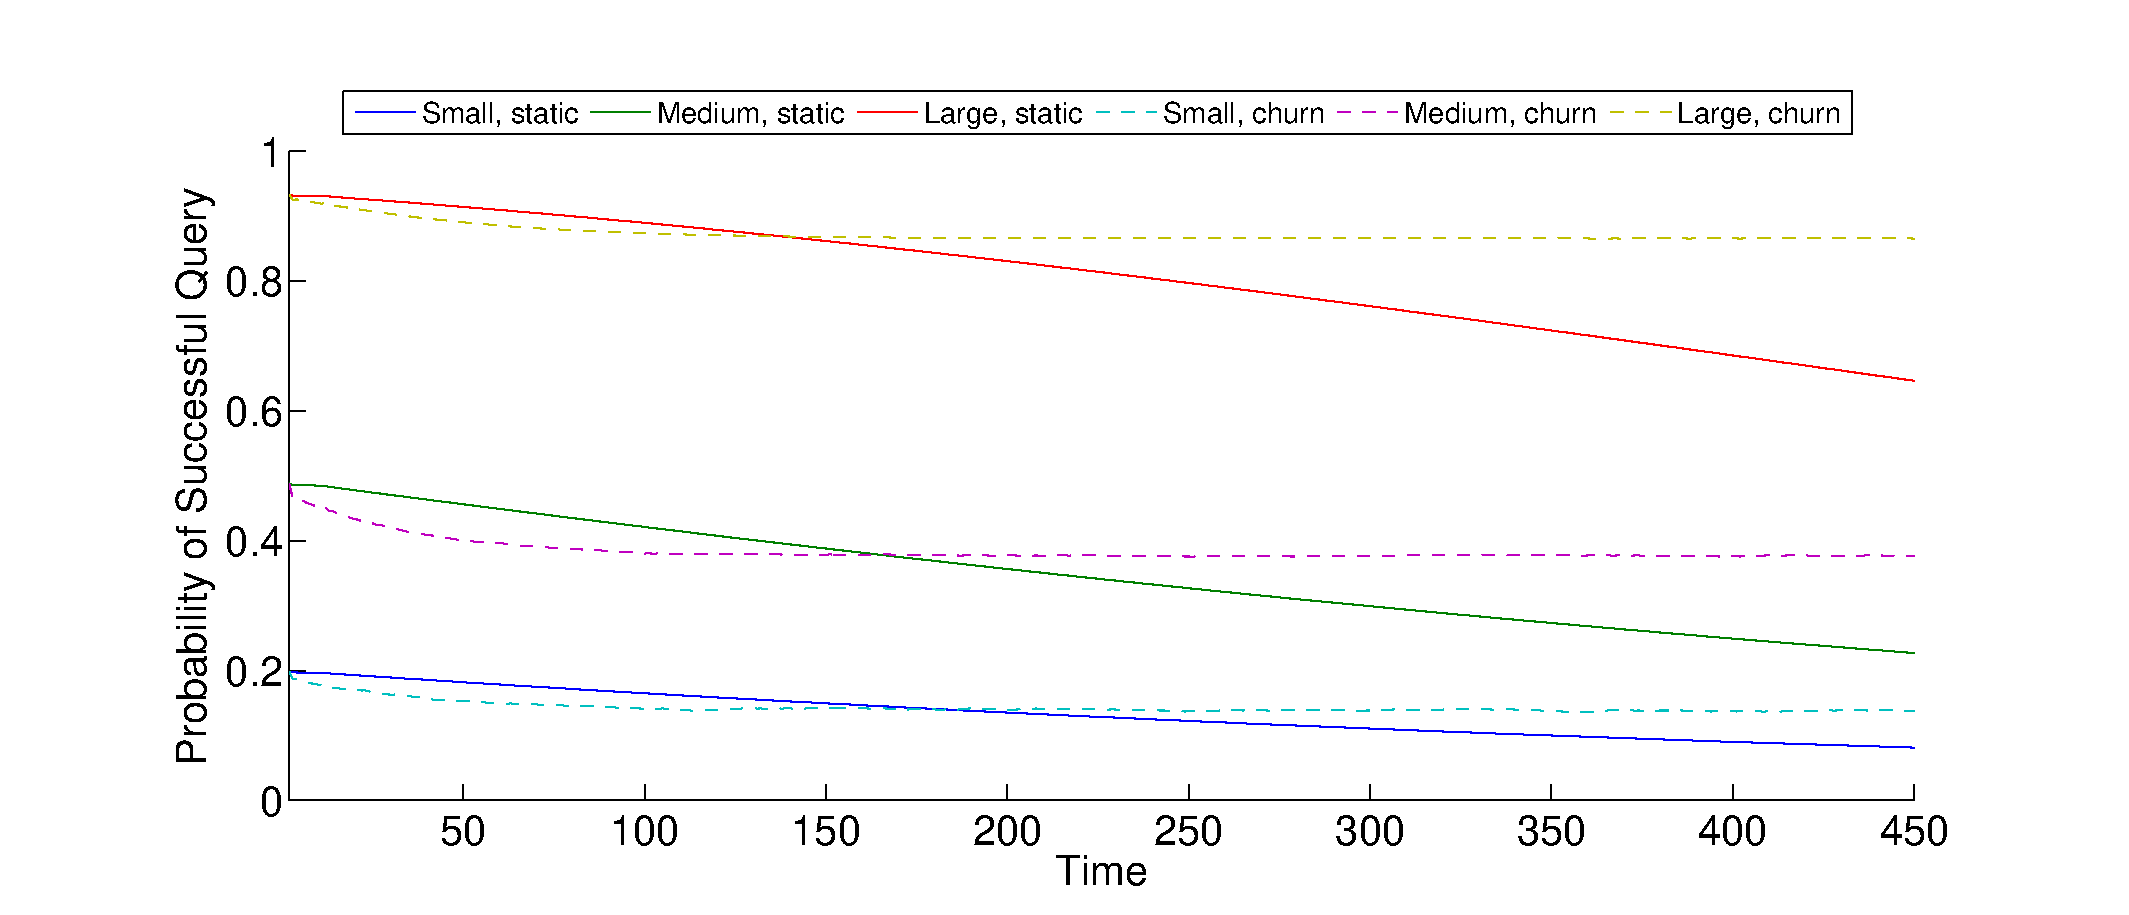
\includegraphics[width=0.5\textwidth]{Images/SimulatedConstant.eps}
        \caption{The probability of succesful search over time for constant model popularities. Both static and churned popularities are shown, for large, medium and small sized torrents.}
        \label{fig:constant_probabilities}
    \end{figure}

%TODO: Graphs display the network scale, shape and PAC strat where needed